\clearpage
\chapter{Harmonic Progression and Function}
\label{sec:harmonic-progression}

\subsection*{What you can do after this chapter}
\begin{itemize}
  \item Classify chords by tonic, subdominant, and dominant function and tell where a chord ``wants'' to go.
  \item Recognise authentic, plagal, half, and deceptive cadences and hear whether a phrase really closes.
  \item Add colour with borrowed chords and secondary dominants, and know why they need resolution.
  \item Modulate with a pivot chord, then lay out the progression in Yeban and hear its bass and functional path.
\end{itemize}

\subsection{Functional harmony: three roles, not three labels}

Function is not a chord's personality. It is the chord's position relative to the tonic and the pull that comes with it. Treat the tonic chord as home; the other chords divide the work of ``leaving home, building tension, and returning'':

\begin{itemize}
  \item \textbf{Tonic function T}: I is the most stable; vi and iii can also support a temporary resting point, with less stability in that order.
  \item \textbf{Subdominant function S}: IV and ii push the ear away from tonic and prepare the dominant.
  \item \textbf{Dominant function D}: V and vii$^\circ$ contain the leading tone or a tritone and naturally resolve back to tonic.
\end{itemize}

In C major, the common chords group like this:

\begin{center}
\small
\begin{tabular}{p{0.10\linewidth}p{0.19\linewidth}p{0.38\linewidth}p{0.21\linewidth}}
\toprule
Function & Role & Common chords in C major & Tendency \\
\midrule
T & tonic & I (C), vi (Am), iii (Em) & stable, resting \\
S & subdominant & IV (F), ii (Dm) & leave tonic, prepare dominant \\
D & dominant & V (G), vii$^\circ$ (Bdim) & tense, waits for resolution \\
\bottomrule
\end{tabular}

Table 6-1. The three functions and their common chords in C major. iii is disputed; it often acts as a weak tonic or a tonic-to-dominant transition.
\end{center}

The classic functional path is \textbf{T → S → D → T}. C--F--G--C is I--IV--V--I: C establishes tonic, F pushes the centre away, G pulls back to C, and C closes. The path is not a law: you may skip S, or substitute vi for I inside the tonic area. But forcing D back into S, such as G--F--C, sounds like going backwards unless that effect is intentional.

Function is not the same as a scale degree. A Roman numeral only marks the root's position in the key; function describes the push that degree carries in context. The same Am is vi (a tonic substitute) in C major but ii (subdominant) in G major. Function without a key is meaningless.

\begin{center}
\begin{minipage}{0.82\linewidth}
\centering
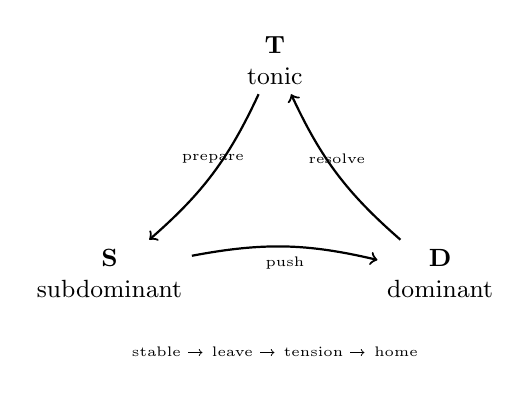
\begin{tikzpicture}[font=\small,every node/.style={align=center}]
  \node (T) at (0,1.7) {\textbf{T}\\ tonic};
  \node (S) at (-2.1,-1.0) {\textbf{S}\\ subdominant};
  \node (D) at (2.1,-1.0) {\textbf{D}\\ dominant};
  \draw[->,thick] (T) to[bend left=12] node[midway,above,font=\tiny]{prepare} (S);
  \draw[->,thick] (S) to[bend left=12] node[midway,below,font=\tiny]{push} (D);
  \draw[->,thick] (D) to[bend left=12] node[midway,above,font=\tiny]{resolve} (T);
  \node[font=\tiny] at (0,-2.0) {stable → leave → tension → home};
\end{tikzpicture}

Figure 6-1. The functional cycle. T establishes the centre, S pushes away, and D pulls back to T.
\end{minipage}
\end{center}

\subsection{Cadences: punctuation at the end of a phrase}

A cadence is a harmonic formula at the end of a phrase. It is not just ``any last two chords''; it tells the ear whether the sentence is finished, unfinished, or deliberately left open. Four common cadences:

\begin{center}
\small
\begin{tabular}{p{0.14\linewidth}p{0.32\linewidth}p{0.42\linewidth}}
\toprule
Type & Example in C major & Sound and use \\
\midrule
Authentic & C--G--C (I--V--I) & clearest close; dominant returns to tonic \\
Plagal & C--F--C (I--IV--I) & soft, broad, like an ``amen'' ending \\
Half & C--Dm--G (I--ii--V) & stops on dominant; phrase continues \\
Deceptive & C--G--Am (I--V--vi) & vi replaces I and delays the close \\
\bottomrule
\end{tabular}

Table 6-2. Four common cadences. Authentic and plagal cadences can be imperfect when inverted or when the melody is not on the tonic.
\end{center}

An authentic cadence is V--I: dominant directly returns to tonic. When V and I are both in root position and the melody lands on the tonic, it is a perfect authentic cadence; an inversion or a melody on the third or fifth makes it less complete. A plagal cadence is IV--I; it has no leading-tone pull, so it sounds softer and more hymn-like. A half cadence stops on V, like a comma. A deceptive cadence substitutes vi for I, releasing some of V's tension without really coming home; it is common when a section needs one more phrase.

Listen to the bass first: V--I moves G→C and is the strongest return; IV--I moves F→C, a gentler version; V--vi moves G→A, a step up, so it does not land. Whether the melody sits on the tonic, third, or fifth also changes how final the cadence feels.

\subsection{Borrowed chords: colour from the parallel minor}

A borrowed chord comes from the parallel mode on the same tonic. C major can borrow from C minor:

\begin{itemize}
  \item \textbf{Fm (iv)}: lower the third of IV and get a darker subdominant; C--Fm--C is heavier than C--F--C.
  \item \textbf{Ab (VI)}: a weighty lower mediant, often placed after C or Fm and resolved back to G or C.
  \item \textbf{Bb (bVII)}: the ``flat seven'' common in rock and folk; it can go straight back to C for a broad bVII--I lift.
  \item \textbf{Cm (i)}: briefly make the tonic minor, switching the major/minor colour on the same root.
\end{itemize}

The key is to return. Fm still belongs to the subdominant area; Ab and Bb usually work as colour and transition. Do not stack a string of borrowed chords without resolution, or the key will fall apart.

\subsection{Secondary dominants: a temporary dominant for a target}

A secondary dominant is the dominant of another chord, written V/X and read ``the dominant of X.'' It treats X temporarily as a local tonic and uses X's leading tone to create local tension:

\begin{itemize}
  \item \textbf{D7 = V/V}: D7 (D--F\sharpsym--A--C) resolves to G. F\sharpsym is G's leading tone and C is G's seventh; together they form a tritone that must resolve.
  \item \textbf{A7 = V/ii}: A7 (A--C\sharpsym--E--G) resolves to Dm; C\sharpsym rises to D.
  \item \textbf{E7 = V/vi}: E7 (E--G\sharpsym--B--D) resolves to Am; G\sharpsym rises to A.
\end{itemize}

Borrowed chords and secondary dominants both introduce chromatic notes, but their sources differ: borrowing looks at another mode on the same tonic; a secondary dominant looks at the dominant of a target chord. The same Ab in C major is usually heard as a borrowed VI; the same D7 can be V/V in C or become V7 when the music modulates to G. Name it by what it resolves to.

\subsection{Modulation: moving the centre}

Modulation is not a change of chord colour; it is a change of the heard tonic. The easiest route is a pivot chord: a chord that exists in both keys, first heard in the old key and then continued in the new one.

C major to G major:

\[
\texttt{C \;\; Am \;\; D7 \;\; G}
\]

\begin{itemize}
  \item C = I in C major, establishing the old tonic.
  \item Am = vi in C major and ii in G major; it is the pivot, still hearable as a tonic substitute in the old key.
  \item D7 = V/V in C major and V7 in G major; it brings out G's leading tone F\sharpsym, and the centre starts to tilt towards G.
  \item G = I in G major; the new tonic stands.
\end{itemize}

\begin{center}
\begin{minipage}{0.92\linewidth}
\centering
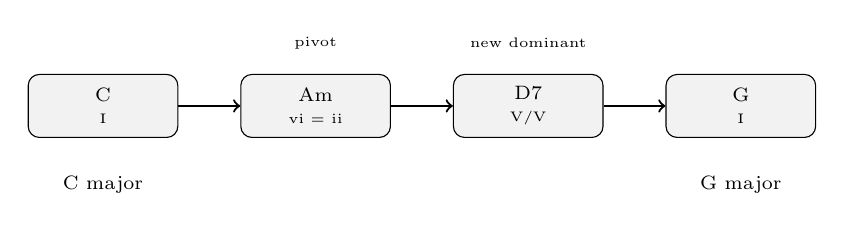
\begin{tikzpicture}[font=\scriptsize,every node/.style={align=center}]
  \node[draw,rounded corners,fill=gray!10,minimum width=1.9cm,minimum height=0.8cm] (c) at (0,0) {C\\ \tiny I};
  \node[draw,rounded corners,fill=gray!10,minimum width=1.9cm,minimum height=0.8cm] (am) at (2.7,0) {Am\\ \tiny vi = ii};
  \node[draw,rounded corners,fill=gray!10,minimum width=1.9cm,minimum height=0.8cm] (d7) at (5.4,0) {D7\\ \tiny V/V};
  \node[draw,rounded corners,fill=gray!10,minimum width=1.9cm,minimum height=0.8cm] (g) at (8.1,0) {G\\ \tiny I};
  \draw[->,thick] (c) -- (am);
  \draw[->,thick] (am) -- (d7);
  \draw[->,thick] (d7) -- (g);
  \node at (0,-1.0) {C major};
  \node at (8.1,-1.0) {G major};
  \node[font=\tiny] at (2.7,0.8) {pivot};
  \node[font=\tiny] at (5.4,0.8) {new dominant};
\end{tikzpicture}

Figure 6-2. The C→G modulation path. Am works in both keys, D7 brings out G's leading tone, and G becomes the new tonic.
\end{minipage}
\end{center}

Whether a modulation succeeds is finally an aural question: is the new tonic actually established, does the melody settle into the new scale, and does the music continue in the new key? One D7 alone often means only a secondary dominant colour; several new-key chords without a new tonic may be no more than vagueness. In writing, use a pivot first, then confirm with the new key's dominant-to-tonic.

\subsection{Common progressions: functions as loops}

Turn functions into a loop and you get a common progression. Four to learn first:

\begin{center}
\small
\begin{tabular}{p{0.20\linewidth}p{0.23\linewidth}p{0.23\linewidth}p{0.23\linewidth}}
\toprule
Progression & In C major/minor & Functional path & Common use \\
\midrule
I--V--vi--IV & C--G--Am--F & T--D--T--S & pop and rock loop \\
ii--V--I & Dm--G--C & S--D--T & jazz close, pop ending \\
i--VI--iv--V & Cm--Ab--Fm--G & T--VI--S--D & minor, Yeban chord lane \\
I--vi--IV--V & C--Am--F--G & T--T--S--D & 1950s pop \\
\bottomrule
\end{tabular}

Table 6-3. Four common progressions. The functional path describes aural tendency, not a rule to follow literally.
\end{center}

The loop of I--V--vi--IV comes from ``tonic, dominant, tonic substitute, subdominant'': vi softens I's stability, IV lifts the centre again, and the return to I both resolves and keeps going. ii--V--I is the jazz close: ii is subdominant, V is dominant, I is tonic; turning the triads into sevenths (Dm7--G7--Cmaj7) makes it smoother. i--VI--iv--V is the minor version; VI and iv both carry subdominant colour, and V uses the major triad of harmonic minor to supply the leading tone. I--vi--IV--V brings vi forward for an earlier ``false close.''

For voice leading, keep common tones and move the rest by the smallest distance; the bass may step or move by fourths and fifths. Do not make every voice leap at once in pursuit of ``advanced'' chords; that blurs the functional path.

\subsection{How to do it in Yeban}

\begin{enumerate}
  \item Open the arrangement area's chord-lane menu item (command \texttt{toggle-chord-lane}), or the expand/collapse toggle above the track headers. A global chord lane appears.
  \item The lane is a fixed five-block demo: \texttt{Cm9}, \texttt{AbMaj7}, \texttt{Fm11}, \texttt{G7\sharpsym9}, and \texttt{Cm11}, with functional labels i9, VI7, iv11, V7\sharpsym9, and i11. Clicking a block or its audition button sends NoteOn/Off to the engine for that chord only; it does not play the whole project.
  \item Listen to the order first: i--VI--iv--V--i, exactly the minor loop of this chapter. Remember that it is a demo and does not follow chords actually written in the project.
  \item To write your own progression, open the piano roll (P/F7) and stack chord tones in the same beat. For ii--V--I in C major: Dm on D4, F4, A4; G on G4, B4, D5; C on C4, E4, G4.
  \item Press Space and listen to the bass first, then the third and fifth. Copy the same bar and change only the last two chords to compare an authentic close with a deceptive one.
  \item To hear the low end alone, use the track header's Solo [S] and keep only the pad or bass track; judge whether the bass is muddy. Do not put all low notes in the same octave.
\end{enumerate}

\screenshot{piano-roll-ii-v-i}{ii–V–I progression laid out in the piano roll}{ii–V–I progression laid out in the piano roll}

\textbf{Scope note:} Yeban currently has no automatic functional analysis, cadence detection, or modulation detection, and no chord-lane editing or ``spell a chord by name'' action. The five chord-lane blocks are fixed demo data, not editable project chords. The audition parser covers only basic triads and common seventh chords: \texttt{Cm9}, \texttt{Fm11}, and \texttt{Cm11} actually sound as minor triads, and \texttt{G7\sharpsym9} actually sounds as a G major triad; 9/11/\sharpsym{}9 extensions are not added automatically. To hear full extensions, stack the notes yourself in the roll. All analysis and modulation decisions here are by ear and on paper; the app does not do them for you.

\subsection{Exercises}

\begin{enumerate}
  \item Classify I, ii, IV, V, and vi in C major by function.
  \par\noindent Answer: I=T, ii=S, IV=S, V=D, vi=T (weak tonic).
  \item Name each cadence: C--G--C; C--F--C; C--Dm--G; C--G--Am.
  \par\noindent Answer: authentic, plagal, half, deceptive.
  \item Write ii--V--I as triads in G major.
  \par\noindent Answer: Am--D--G.
  \item Where do Fm, Ab, and Bb in C major come from, and what colour does each add?
  \par\noindent Answer: borrowed from C minor as iv, VI, and bVII; Fm darkens the subdominant, Ab adds weight, Bb broadens and can return directly to C.
  \item Which chord is the pivot in C--Am--D7--G, and what key does it lead to?
  \par\noindent Answer: Am (vi in C and ii in G); it leads to G major, with D7 as G's V7.
  \item In Yeban's chord lane, click Cm9, AbMaj7, Fm11, G7\sharpsym9, and Cm11 in order. Write the functional path, and explain why G7\sharpsym9 does not sound its \sharpsym{}9.
  \par\noindent Answer: i--VI--iv--V--i; the audition parser stops at basic triads/sevenths, so \texttt{G7\sharpsym9} actually sounds as a G major triad and the extension is not added automatically (see the scope note in Chapter 5 and issue \texttt{ISS-MWW4F0LZ-C8939F}).
\end{enumerate}

\subsection{Help topic map}

\begin{center}
\footnotesize
\begin{tabular}{p{0.22\linewidth}p{0.54\linewidth}p{0.16\linewidth}}
\toprule
Section & In-app help anchor & Note \\
\midrule
Functional harmony & \texttt{music-theory-harmonic-function} & concept \\
Cadences & \texttt{music-theory-cadences} & Table 6-2 \\
Borrowed and secondary & \texttt{music-theory-borrowed-secondary} & colour / resolution \\
Modulation & \texttt{music-theory-modulation} & Figure 6-2 \\
Common progressions & \texttt{music-theory-functional-progressions} & Table 6-3 \\
Bass and voicing & \texttt{music-theory-bass-voicing} & arrangement \\
How to in Yeban & \texttt{music-theory-piano-roll-progressions} & operation \\
Exercises & \texttt{music-theory-ch6-practice} & answers at chapter end \\
\bottomrule
\end{tabular}
\end{center}
